\chapter{Perancangan}

\section{Perancangan Antarmuka}
Dalam perangkat lunak yang dibangun, tampilan yang digunakan adalah tampilan antarmuka grafis. Tampilan antarmuka ini berguna untuk mempermudah interaksi pengguna dengan perangkat lunak. Selain mempermudah, tampilan ini digunakan agar dapat menghasilkan visualisasi penempatan kamera CCTV sehingga pengguna dapat memahami penempatan-penempatan tersebut. Pada bagian ini akan dijelaskan bentuk dari setiap antarmuka. Berikut bentuk antarmuka-antarmuka tersebut:

\begin{itemize}
	\item Antarmuka: \textbf{Penerima Masukan}\\
	Antarmuka ini berfungsi untuk menerima masukan dari pengguna. Antarmuka ini dapat dilihat pada gambar~\ref{fig:input_mockup}. Pada antarmuka ini terdapat kolom-kolom masukan yang dapat diisi oleh pengguna. Pengguna dapat mengisi ukuran ruangan, spesifikasi kamera CCTV, dan ukuran terbesar cell pada kolom-kolom tersebut. Apabila pengguna sudah yakin dengan masukannya, maka pengguna dapat menekan tombol ''\textit{submit}'' yang akan mengarahkan pengguna pada antarmuka simulasi penempatan kamera CCTV.
	\begin{figure}[h]
		\centering  
		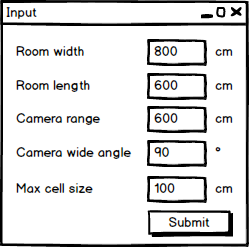
\includegraphics[scale=0.6]{input_mockup}
		\caption[Perancangan antarmuka penerima masukan]{Perancangan antarmuka penerima masukan}
		\label{fig:input_mockup}
	\end{figure}

	\item Antarmuka: \textbf{Simulasi Penempatan Kamera CCTV}\\
	Antarmuka ini berfungsi untuk melakukan kegiatan simulasi penempatan kamera CCTV. Antarmuka ini dapat dilihat pada gambar~\ref{fig:simulator_mockup}. Di dalam antarmuka ini terdapat 3 bagian, yaitu:
	\begin{itemize}
		\item Panel informasi yang berada di bagian kiri antarmuka.\\
		Panel ini berfungsi untuk memberikan informasi-informasi yang terdiri dari ukuran ruangan, spesifikasi kamera CCTV, informasi simulasi, dan daftar penempatan kamera CCTV. Pada bagian informasi simulasi terdapat informasi persentase ketercakupan dan persentase tingkat \textit{overlap} dan \textit{out of bound}. Pada bagian daftar penempatan kamera CCTV, terdapat penempatan-penempatan yang sedang diterapkan dalam simulasi. Pada setiap penempatan terdapat tombol ''\textit{remove}'' yang apabila ditekan akan membuang penempatan tersebut.
		
		\item Panel visualisasi penempatan kamera CCTV yang berada di bagian kanan antarmuka.\\
		Panel ini berfungsi untuk menampilkan visualisasi penempatan kamera CCTV sesuai dengan penempatan-penempatan yang sedang diterapkan pada simulasi.
		
		\item Panel penambah kamera CCTV yang berada di atas panel visualisasi.\\
		Panel ini berfungsi untuk melakukan penempatan kamera CCTV baru. Pengguna dapat melakukan 2 jenis penambahan penempatan, yaitu penambahan sesuai dengan keinginan pengguna dan penambahan secara otomatis. Apabila pengguna ingin melakukan penambahan sesuai dengan keinginan, maka pengguna dapat memilih posisi dan mengisi sudut arah pandang dan dilanjutkan dengan menekan tombol ''\textit{add camera}''. Apabila pengguna ingin melakukan penambahan secara otomatis, maka pengguna dapat menekan tombol ''\textit{auto place camera}''. Dengan melakukan penambahan secara otomatis, sistem akan mencari penempatan-penempatan tersedikit yang dapat mencakup seluruh cell yang belum tercakup. Selama proses penambahan otomatis berjalan, tombol ''\textit{add camera}'' dan tombol ''\textit{auto place camera}'' akan dinon-aktifkan dan diaktifkan kembali apabila proses telah selesai.
	\end{itemize}
	\begin{figure}[h]
		\centering  
		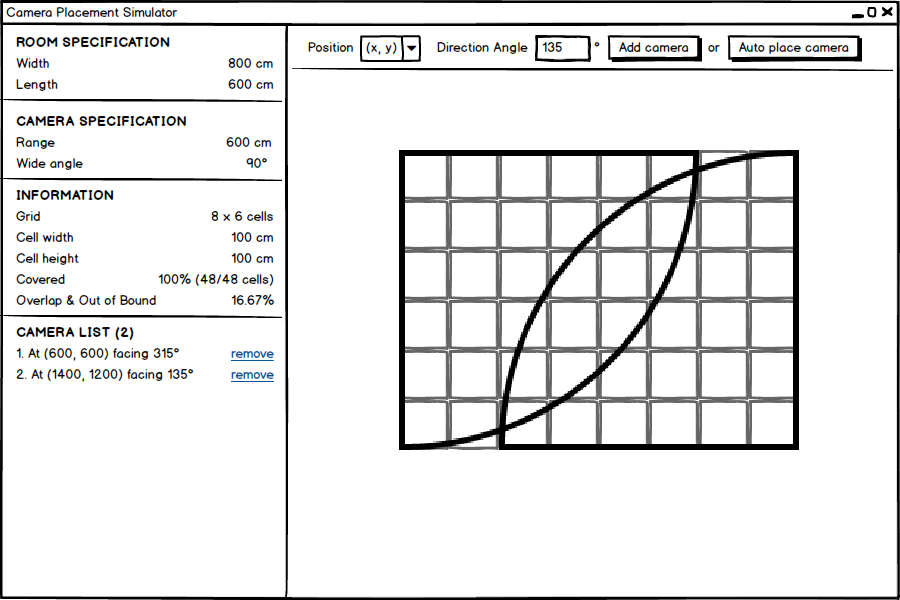
\includegraphics[scale=0.5]{simulator_mockup}
		\caption[Perancangan antarmuka penempatan kamera CCTV]{Perancangan antarmuka penempatan kamera CCTV}
		\label{fig:simulator_mockup}
	\end{figure}
\end{itemize}

\section{Perancangan Kelas}
Pada bagian ini akan dijelaskan kelas-kelas yang digunakan dalam membangun perangkat lunak. Diagram kelas rinci dapat dilihat pada gambar~\ref{fig:class_diagram_complete}.
\begin{sidewaysfigure}
	\centering  
	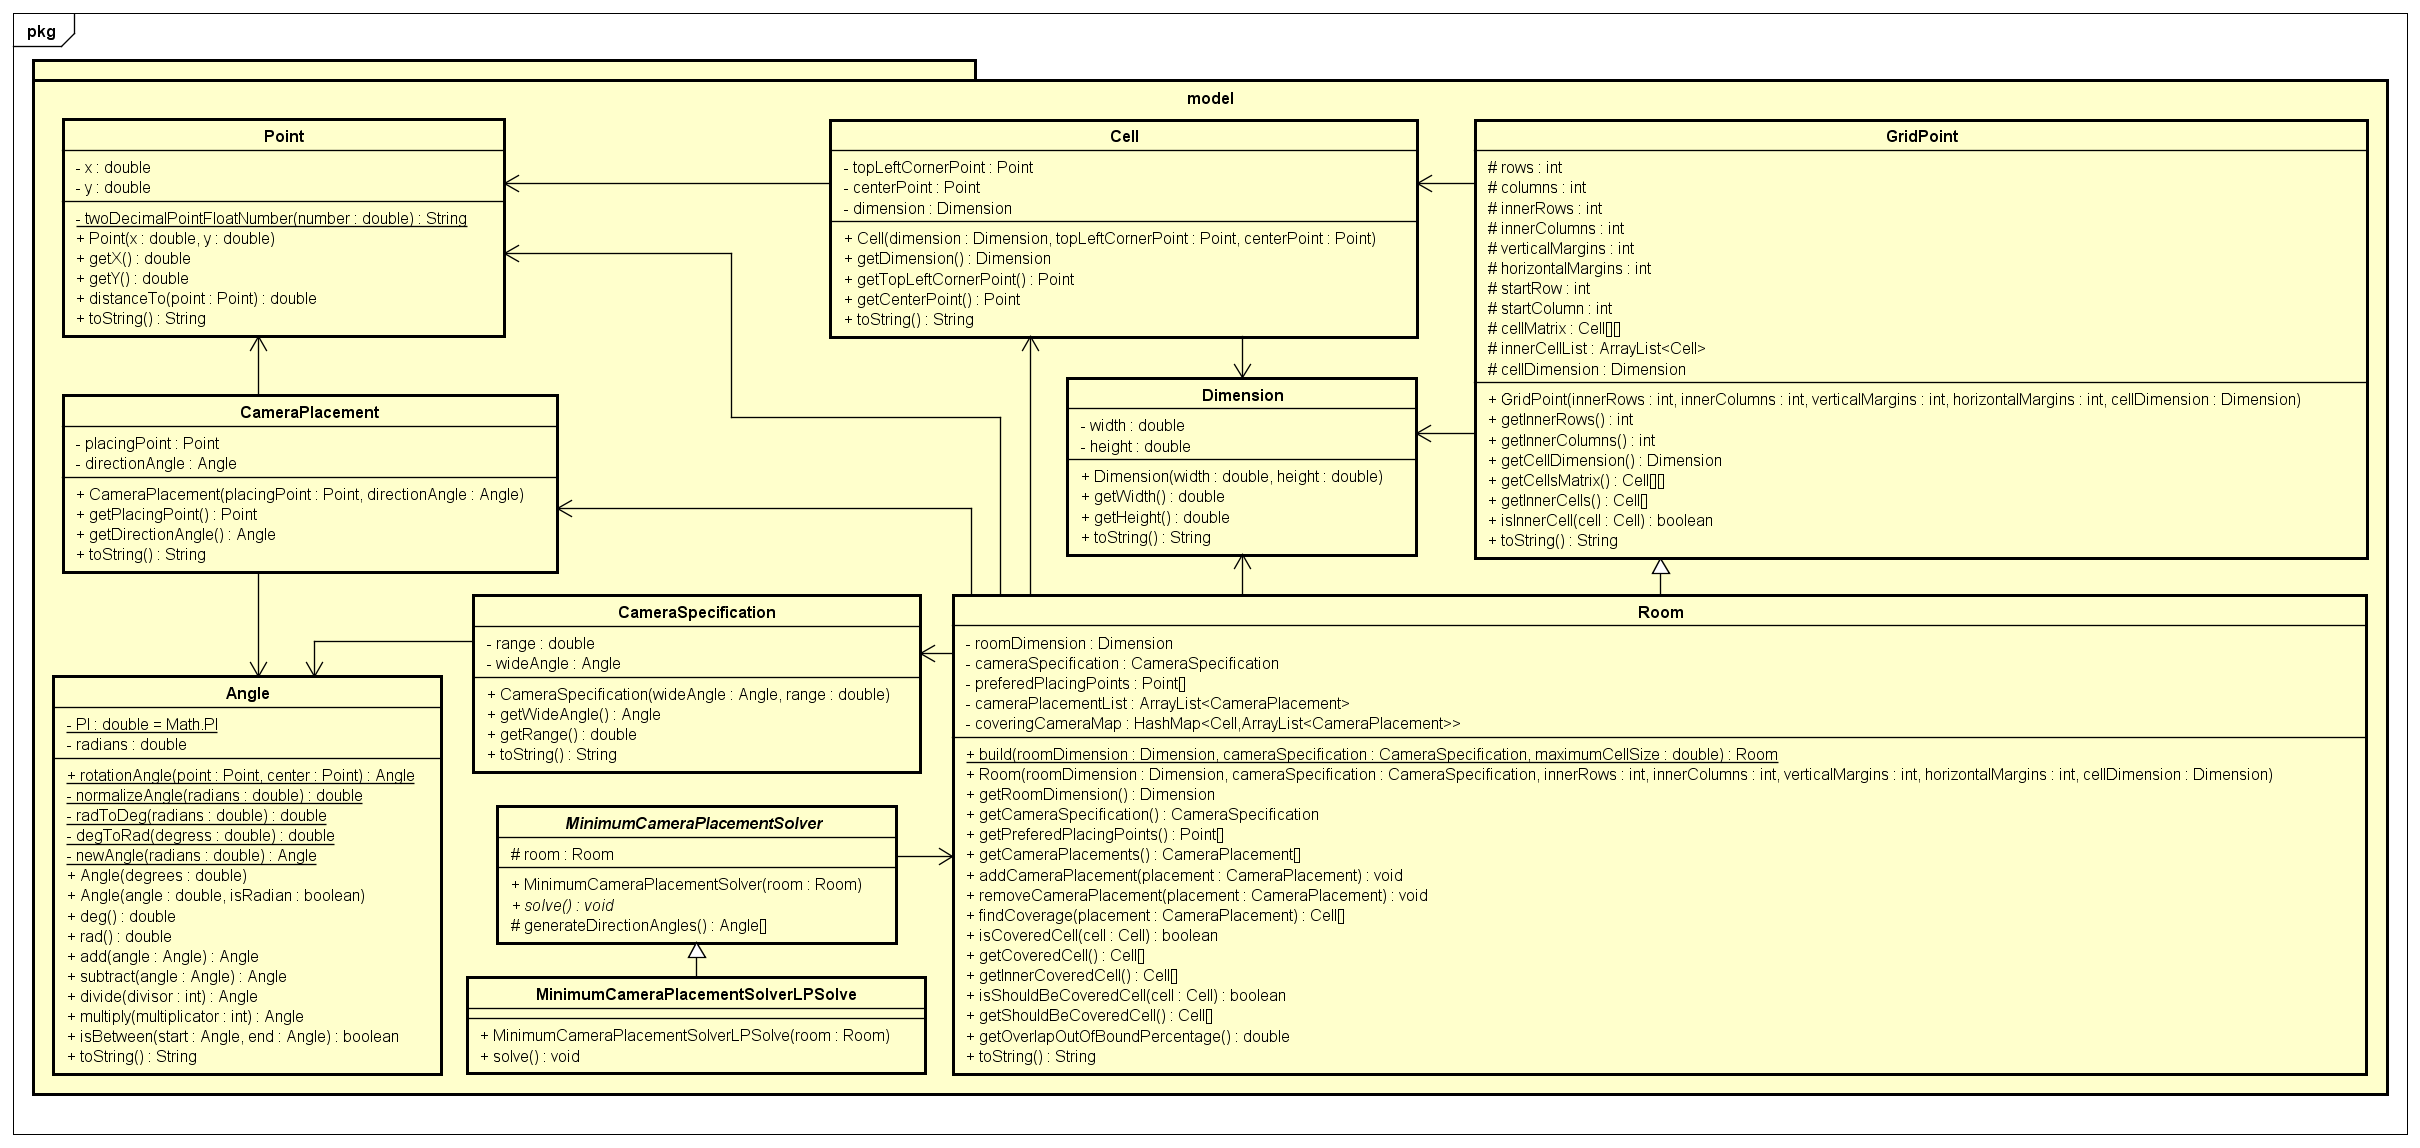
\includegraphics[scale=0.38]{class_diagram_complete}
	\caption[Diagram kelas rinci]{Diagram kelas rinci}
	\label{fig:class_diagram_complete}
\end{sidewaysfigure}

\subsection{Kelas \textit{Angle}}
\begin{figure}[H]
	\centering  
	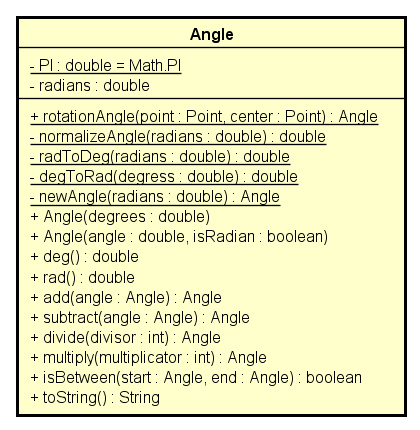
\includegraphics[scale=0.6]{class_angle}
	\caption[Diagram kelas \textit{Angle}]{Diagram kelas \textit{Angle}}
	\label{fig:class_angle}
\end{figure}
	
Kelas ini merepresentasikan sudut dan menangani fungsi-fungsi yang berhubungan dengan sudut. Diagram kelas \textit{Angle} dapat dilihat pada gambar~\ref{fig:class_angle}. Berikut ini merupakan atribut-atribut yang terdapat pada kelas \textit{Angle}:
\begin{itemize}
	\item \textbf{\textit{PI} \(\rightarrow\) \textit{double}}\\
	Atribut ini merupakan atribut statis bernilai \(\pi\) yang dapat digunakan oleh setiap objek dari kelas \textit{Angle}.
	\item \textbf{\textit{radians} \(\rightarrow\) \textit{double}}\\
	Atribut ini berguna untuk menampung sudut dalam bentuk radian.
\end{itemize}

Berikut ini merupakan fungsi-fungsi yang terdapat pada kelas \textit{Angle}:
\begin{itemize}
	\item \textbf{\textit{rotationAngle}(\textit{point} \(\rightarrow\) \textit{Point}, \textit{center} \(\rightarrow\) \textit{Point}) \(\rightarrow\) \textit{Angle}}\\
	Fungsi ini merupakan fungsi statis yang berguna untuk mendapatkan sudut rotasi dari titik \textit{point} terhadap titik \textit{center}.
	\item \textbf{\textit{normalizeAngle}(\textit{radians} \(\rightarrow\) \textit{double}) \(\rightarrow\) \textit{double}}\\
	Fungsi ini merupakan fungsi statis yang berguna untuk melakukan normalisasi sudut \textit{radians} sehingga berada dalam rentang \(0\leq\textit{radians}<2\pi\).
	\item \textbf{\textit{radToDeg}(\textit{radians} \(\rightarrow\) \textit{double}) \(\rightarrow\) \textit{double}}\\
	Fungsi ini merupakan fungsi statis yang berguna untuk mengubah sudut dalam bentuk radian menjadi sudut dalam bentuk derajat.
	\item \textbf{\textit{degToRad}(\textit{degrees} \(\rightarrow\) \textit{double}) \(\rightarrow\) \textit{double}}\\
	Fungsi ini merupakan fungsi statis yang berguna untuk mengubah sudut dalam bentuk derajat menjadi sudut dalam bentuk radian.
	\item \textbf{\textit{newAngle}(\textit{radians} \(\rightarrow\) \textit{double}) \(\rightarrow\) \textit{Angle}}\\
	Fungsi ini merupakan fungsi statis yang berguna untuk membuat objek \textit{Angle} baru.
	\item \textbf{\textit{deg}() \(\rightarrow\) \textit{double}}\\
	Fungsi ini berguna untuk mendapatkan sudut dalam bentuk derajat.
	\item \textbf{\textit{rad}() \(\rightarrow\) \textit{double}}\\
	Fungsi ini berguna untuk mendapatkan sudut dalam bentuk radian.
	\item \textbf{\textit{add}(\textit{angle} \(\rightarrow\) \textit{Angle}) \(\rightarrow\) \textit{Angle}}\\
	Fungsi ini berguna untuk menghasilkan objek sudut baru yang merupakan hasil penjumlahan antara sudut objek ini dengan sudut objek \textit{angle}.
	\item \textbf{\textit{subtract}(\textit{angle} \(\rightarrow\) \textit{Angle}) \(\rightarrow\) \textit{Angle}}\\
	Fungsi ini berguna untuk menghasilkan objek sudut baru yang merupakan hasil pengurangan antara sudut objek ini dengan sudut objek \textit{angle}.
	\item \textbf{\textit{divide}(\textit{divisor} \(\rightarrow\) \textit{int}) \(\rightarrow\) \textit{Angle}}\\
	Fungsi ini berguna untuk menghasilkan objek sudut baru yang merupakan hasil pembagian antara sudut objek ini dengan nilai \textit{divisor}.
	\item \textbf{\textit{multiply}(\textit{multiplicator} \(\rightarrow\) \textit{int}) \(\rightarrow\) \textit{Angle}}\\
	Fungsi ini berguna untuk menghasilkan objek sudut baru yang merupakan hasil pengalian antara sudut objek ini dengan nilai \textit{multiplicator}.
	\item \textbf{\textit{isBetween}(\textit{start} \(\rightarrow\) \textit{Angle}, \textit{end} \(\rightarrow\) \textit{Angle}) \(\rightarrow\) \textit{boolean}}\\
	Fungsi ini berguna untuk mengetahui apakah sudut objek ini berada di antara sudut objek \textit{start} dan sudut objek \textit{end}.
\end{itemize}

\subsection{Kelas \textit{Point}}
\begin{figure}[H]
	\centering  
	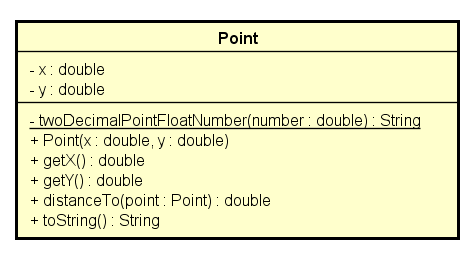
\includegraphics[scale=0.6]{class_point}
	\caption[Diagram kelas \textit{Point}]{Diagram kelas \textit{Point}}
	\label{fig:class_point}
\end{figure}

Kelas ini merepresentasikan titik koordinat 2D. Diagram kelas \textit{Point} dapat dilihat pada gambar~\ref{fig:class_point}. Berikut ini merupakan atribut-atribut yang terdapat pada kelas \textit{Point}:
\begin{itemize}
	\item \textbf{\textit{x} \(\rightarrow\) \textit{double}}\\
	Atribut ini berguna untuk menampung nilai titik pada sumbu x.
	\item \textbf{\textit{y} \(\rightarrow\) \textit{double}}\\
	Atribut ini berguna untuk menampung nilai titik pada sumbu y.
\end{itemize}

Berikut ini merupakan fungsi-fungsi yang terdapat pada kelas \textit{Point}:
\begin{itemize}
	\item \textbf{\textit{twoDecimalPointFloatNumber}(\textit{number} \(\rightarrow\) \textit{double}) \(\rightarrow\) \textit{String}}\\
	Fungsi ini merupakan fungsi statis yang berguna untuk mengubah bilangan \textit{number} ke dalam bentuk \textit{String} dengan maksimal bilangan di belakang koma berjumlah 2 buah.
	\item \textbf{\textit{distanceTo}(\textit{point} \(\rightarrow\) \textit{Point}) \(\rightarrow\) \textit{double}}\\
	Fungsi ini berguna untuk mendapatkan jarak antara titik objek ini dengan titik objek \textit{point}.
\end{itemize}

\subsection{Kelas \textit{CameraSpecification}}
\begin{figure}[H]
	\centering  
	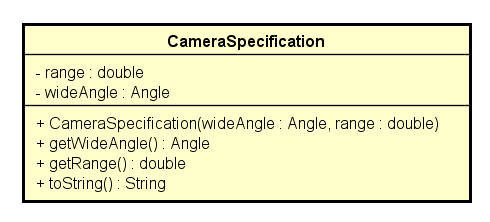
\includegraphics[scale=0.6]{class_camera_specification}
	\caption[Diagram kelas \textit{CameraSpecification}]{Diagram kelas \textit{CameraSpecification}}
	\label{fig:class_camera_specification}
\end{figure}

Kelas ini merepresentasikan spesifikasi kamera CCTV yang terdiri dari jarak pandang efektif dan besar sudut pandang. Diagram kelas \textit{CameraSpecification} dapat dilihat pada gambar~\ref{fig:class_camera_specification}. Berikut ini merupakan atribut-atribut yang terdapat pada kelas \textit{CameraSpecification}:
\begin{itemize}
	\item \textbf{\textit{range} \(\rightarrow\) \textit{double}}\\
	Atribut ini berguna untuk menampung jarak pandang efektif kamera CCTV.
	\item \textbf{\textit{wideAngle} \(\rightarrow\) \textit{Angle}}\\
	Atribut ini berguna untuk menampung besar sudut pandang kamera CCTV.
\end{itemize}

\subsection{Kelas \textit{CameraPlacement}}
\begin{figure}[H]
	\centering  
	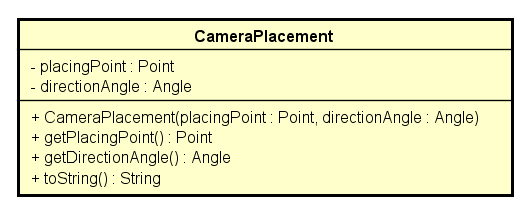
\includegraphics[scale=0.6]{class_camera_placement}
	\caption[Diagram kelas \textit{CameraPlacement}]{Diagram kelas \textit{CameraPlacement}}
	\label{fig:class_camera_placement}
\end{figure}

Kelas ini merepresentasikan penempatan kamera CCTV yang terdiri dari posisi dan sudut arah pandang. Diagram kelas \textit{CameraPlacement} dapat dilihat pada gambar~\ref{fig:class_camera_placement}. Berikut ini merupakan atribut-atribut yang terdapat pada kelas \textit{CameraPlacement}:
\begin{itemize}
	\item \textbf{\textit{placingPoint} \(\rightarrow\) \textit{Point}}\\
	Atribut ini berguna untuk menampung posisi penempatan kamera CCTV.
	\item \textbf{\textit{directionAngle} \(\rightarrow\) \textit{Angle}}\\
	Atribut ini berguna untuk menampung sudut arah pandang kamera CCTV.
\end{itemize}

\subsection{Kelas \textit{Dimension}}
\begin{figure}[H]
	\centering  
	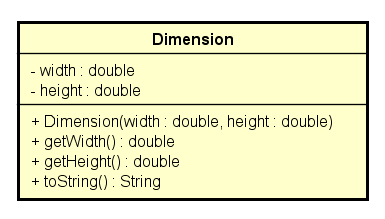
\includegraphics[scale=0.6]{class_dimension}
	\caption[Diagram kelas \textit{Dimension}]{Diagram kelas \textit{Dimension}}
	\label{fig:class_dimension}
\end{figure}

Kelas ini merepresentasikan dimensi yang terdiri dari panjang dan lebar. Diagram kelas \textit{Dimension} dapat dilihat pada gambar~\ref{fig:class_dimension}. Berikut ini merupakan atribut-atribut yang terdapat pada kelas \textit{Dimension}:
\begin{itemize}
	\item \textbf{\textit{width} \(\rightarrow\) \textit{double}}\\
	Atribut ini berguna untuk menampung ukuran lebar.
	\item \textbf{\textit{length} \(\rightarrow\) \textit{double}}\\
	Atribut ini berguna untuk menampung ukuran panjang.
\end{itemize}

\subsection{Kelas \textit{Cell}}
\begin{figure}[H]
	\centering  
	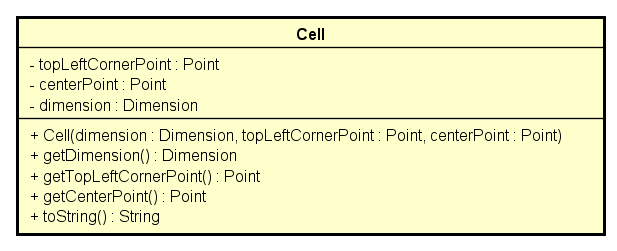
\includegraphics[scale=0.6]{class_cell}
	\caption[Diagram kelas \textit{Cell}]{Diagram kelas \textit{Cell}}
	\label{fig:class_cell}
\end{figure}

Kelas ini merepresentasikan cell. Diagram kelas \textit{Cell} dapat dilihat pada gambar~\ref{fig:class_cell}. Berikut ini merupakan atribut-atribut yang terdapat pada kelas \textit{Cell}:
\begin{itemize}
	\item \textbf{\textit{topLeftCornerPoint} \(\rightarrow\) \textit{Point}}\\
	Atribut ini berguna untuk menampung titik ujung kiri atas cell.
	\item \textbf{\textit{centerPoint} \(\rightarrow\) \textit{Point}}\\
	Atribut ini berguna untuk menampung titik tengah cell.
	\item \textbf{\textit{dimension} \(\rightarrow\) \textit{Dimension}}\\
	Atribut ini berguna untuk menampung dimensi cell.
\end{itemize}

\subsection{Kelas \textit{GridPoint}}
\begin{figure}[H]
	\centering  
	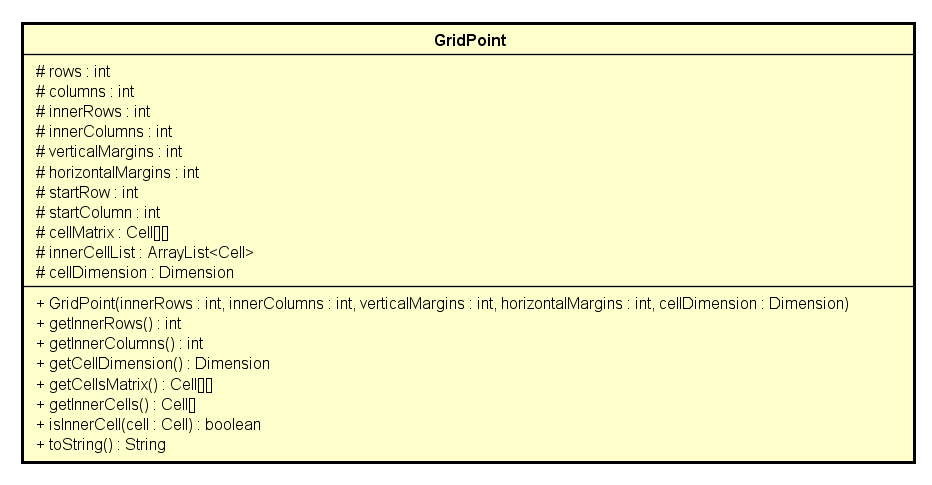
\includegraphics[scale=0.6]{class_grid_point}
	\caption[Diagram kelas \textit{GridPoint}]{Diagram kelas \textit{GridPoint}}
	\label{fig:class_grid_point}
\end{figure}

Kelas ini merepresentasikan grid point yang terdiri dari matriks cell. Diagram kelas \textit{GridPoint} dapat dilihat pada gambar~\ref{fig:class_grid_point}. Berikut ini merupakan atribut-atribut yang terdapat pada kelas \textit{GridPoint}:
\begin{itemize}
	\item \textbf{\textit{rows} \(\rightarrow\) \textit{int}}\\
	Atribut ini berguna untuk menampung jumlah baris grid point secara keseluruhan.
	\item \textbf{\textit{columns} \(\rightarrow\) \textit{int}}\\
	Atribut ini berguna untuk menampung jumlah kolom grid point secara keseluruhan.
	\item \textbf{\textit{innerRows} \(\rightarrow\) \textit{int}}\\
	Atribut ini berguna untuk menampung jumlah baris grid point bagian dalam.
	\item \textbf{\textit{innerColumns} \(\rightarrow\) \textit{int}}\\
	Atribut ini berguna untuk menampung jumlah kolom grid point bagian dalam.
	\item \textbf{\textit{verticalMargins} \(\rightarrow\) \textit{int}}\\
	Atribut ini berguna untuk menampung jumlah margin vertikal grid point.
	\item \textbf{\textit{horizontalMargins} \(\rightarrow\) \textit{int}}\\
	Atribut ini berguna untuk menampung jumlah margin horizontal grid point.
	\item \textbf{\textit{startRow} \(\rightarrow\) \textit{int}}\\
	Atribut ini berguna untuk menampung indeks baris pertama dalam grid point bagian dalam.
	\item \textbf{\textit{startColumn} \(\rightarrow\) \textit{int}}\\
	Atribut ini berguna untuk menampung indeks kolom pertama dalam grid point bagian dalam.
	\item \textbf{\textit{cellMatrix} \(\rightarrow\) \textit{Cell}[ ][ ]}\\
	Atribut ini berguna untuk menampung matriks cell 2 dimensi.
	\item \textbf{\textit{innerCellList} \(\rightarrow\) \textit{ArrayList}<\textit{Cell}>}\\
	Atribut ini berguna untuk menampung cell-cell yang berada pada grid point bagian dalam.
	\item \textbf{\textit{cellDimension} \(\rightarrow\) \textit{Dimension}}\\
	Atribut ini berguna untuk menampung dimensi cell.
\end{itemize}

\subsection{Kelas \textit{Room}}
\begin{figure}[H]
	\centering  
	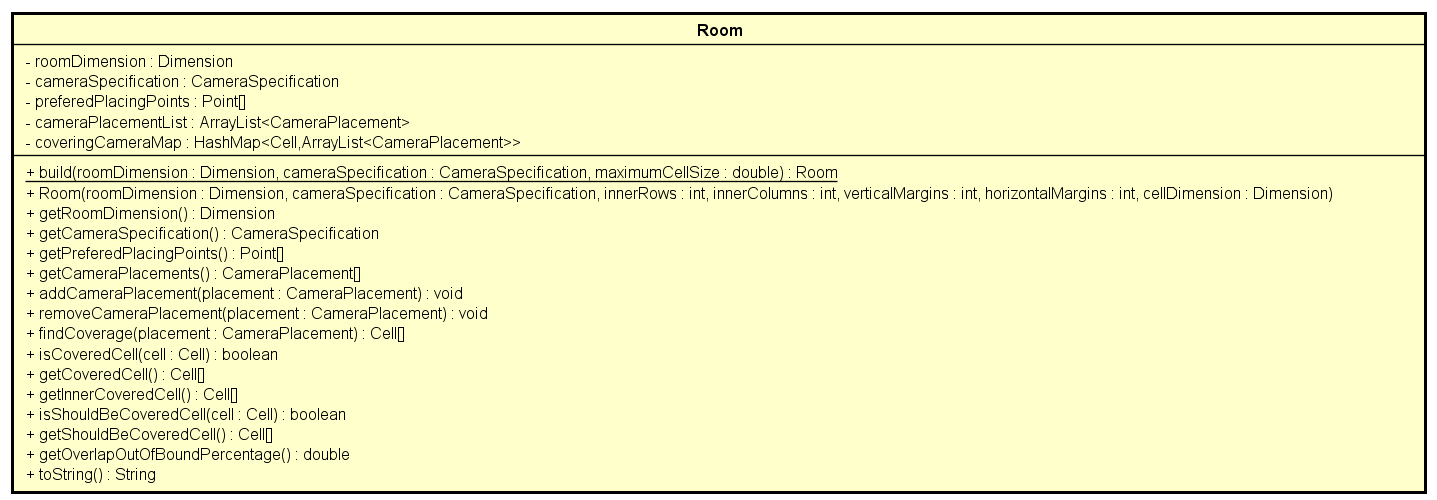
\includegraphics[scale=0.4]{class_room}
	\caption[Diagram kelas \textit{Room}]{Diagram kelas \textit{Room}}
	\label{fig:class_room}
\end{figure}

Kelas ini merepresentasikan ruangan yang dapat diisi oleh kamera-kamera CCTV. Kelas ini merupakan turunan dari kelas \textit{GridPoint}. Diagram kelas \textit{Room} dapat dilihat pada gambar~\ref{fig:class_room}. Berikut ini merupakan atribut-atribut yang terdapat pada kelas \textit{Room}:
\begin{itemize}
	\item \textbf{\textit{roomDimension} \(\rightarrow\) \textit{Dimension}}\\
	Atribut ini berguna untuk menampung dimensi ruangan.
	\item \textbf{\textit{cameraSpecification} \(\rightarrow\) \textit{CameraSpecification}}\\
	Atribut ini berguna untuk menampung spesifikasi kamera CCTV yang akan ditempatkan dalam ruangan.
	\item \textbf{\textit{preferedPlacingPoints} \(\rightarrow\) \textit{Point}[ ]}\\
	Atribut ini berguna untuk menampung posisi-posisi yang dapat ditempati oleh kamera CCTV.
	\item \textbf{\textit{cameraPlacementList} \(\rightarrow\) \textit{ArrayList}<\textit{CameraPlacement}>}\\
	Atribut ini berguna untuk menampung daftar penempatan kamera CCTV.
	\item \textbf{\textit{coveringCameraMap} \(\rightarrow\) \textit{HashMap}<\textit{Cell}, \textit{ArrayList}{<\textit{CameraPlacement}>}>}\\
	Atribut ini berguna untuk menampung pemetaan cell dengan penempatan-penempatan kamera CCTV yang dapat mencakup cell tersebut.
\end{itemize}

Berikut ini merupakan fungsi-fungsi yang terdapat pada kelas \textit{Room}:
\begin{itemize}
	\item \textbf{\textit{build}(\textit{roomDimension} \(\rightarrow\) \textit{Dimension}, \textit{cameraSpecification} \(\rightarrow\) \textit{CameraSpecification}, \textit{maximumCellSize} \(\rightarrow\) \textit{double}) \(\rightarrow\) \textit{Room}}\\
	Fungsi ini merupakan fungsi statis yang berguna untuk membuat objek \textit{Room} yang dimana jumlah baris, jumlah kolom, jumlah margin vertikal, jumlah margin horizontal, dan ukuran cell akan ditentukan berdasarkan ukuran ruangan \textit{roomDimension}, spesifikasiKamera \textit{cameraSpecification}, dan ukuran terbesar cell \textit{maximumCellSize}.
	\item \textbf{\textit{addCameraPlacement}(\textit{placement} \(\rightarrow\) \textit{CameraPlacement}) \(\rightarrow\) \textit{void}}\\
	Fungsi ini berguna untuk menambahkan penempatan kamera CCTV ke dalam daftar penempatan kamera CCTV dan memperbaharui pemetaan cell pada atribut \textit{coveringCameraMap}.
	\item \textbf{\textit{removeCameraPlacement}(\textit{placement} \(\rightarrow\) \textit{CameraPlacement}) \(\rightarrow\) \textit{void}}\\
	Fungsi ini berguna untuk membuang penempatan kamera CCTV dari daftar penempatan kamera CCTV dan memperbaharui pemetaan cell pada atribut \textit{coveringCameraMap}.
	\item \textbf{\textit{findCoverage}(\textit{placement} \(\rightarrow\) \textit{CameraPlacement}) \(\rightarrow\) \textit{Cell}[ ]}\\
	Fungsi ini berguna untuk mendapatkan cell-cell yang tercakup oleh penempatan \textit{placement}.
	\item \textbf{\textit{isCoveredCell}(\textit{cell} \(\rightarrow\) \textit{Cell}) \(\rightarrow\) \textit{boolean}}\\
	Fungsi ini berguna untuk mengetahui apakah cell \textit{cell} telah tercakup oleh setidaknya 1 penempatan kamera CCTV.
	\item \textbf{\textit{getCoveredCell}() \(\rightarrow\) \textit{Cell}[ ]}\\
	Fungsi ini berguna untuk mendapatkan cell-cell yang telah tercakup oleh setidaknya 1 penempatan kamera CCTV.
	\item \textbf{\textit{getInnerCoveredCell}() \(\rightarrow\) \textit{Cell}[ ]}\\
	Fungsi ini berguna untuk mendapatkan cell-cell yang berada pada grid point bagian dalam dan telah tercakup oleh setidaknya 1 penempatan kamera CCTV.
	\item \textbf{\textit{isShouldBeCoveredCell}(\textit{cell} \(\rightarrow\) \textit{Cell}) \(\rightarrow\) \textit{boolean}}\\
	Fungsi ini berguna untuk mengetahui apakah cell \textit{cell} berada pada grid point bagian dalam dan belum tercakup oleh setidaknya 1 penempatan kamera CCTV.
	\item \textbf{\textit{getShouldBeCoveredCell}() \(\rightarrow\) \textit{Cell}[ ]}\\
	Fungsi ini berguna untuk mendapatkan cell-cell yang berada pada grid point bagian dalam dan belum tercakup oleh setidaknya 1 penempatan kamera CCTV.
	\item \textbf{\textit{getOverlapAndOutOfBoundPercentage}() \(\rightarrow\) \textit{double}}\\
	Fungsi ini berguna untuk mendapatkan persentase \textit{overlap} dan \textit{out of bound}.
\end{itemize}

\subsection{Kelas \textit{MinimumCameraPlacementSolver}}
\begin{figure}[H]
	\centering  
	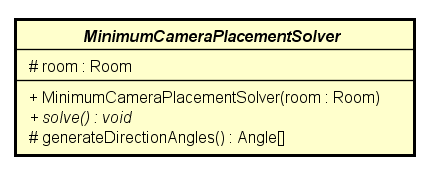
\includegraphics[scale=0.6]{class_minimum_camera_placement_solver}
	\caption[Diagram kelas \textit{MinimumCameraPlacementSolver}]{Diagram kelas \textit{MinimumCameraPlacementSolver}}
	\label{fig:class_minimum_camera_placement_solver}
\end{figure}

Kelas ini merepresentasikan pemecah masalah penempatan kamera CCTV dalam ruangan agar berjumlah minimum. Kelas ini merupakan kelas abstrak. Diagram kelas \textit{MinimumCameraPlacementSolver} dapat dilihat pada gambar~\ref{fig:class_minimum_camera_placement_solver}. Berikut ini merupakan atribut-atribut yang terdapat pada kelas \textit{MinimumCameraPlacementSolver}:
\begin{itemize}
	\item \textbf{\textit{room} \(\rightarrow\) \textit{Room}}\\
	Atribut ini berguna untuk menampung ruangan yang akan diselesaikan masalahnya.
\end{itemize}

Berikut ini merupakan fungsi-fungsi yang terdapat pada kelas \textit{Room}:
\begin{itemize}
	\item \textbf{\textit{solve}() \(\rightarrow\) \textit{void}}\\
	Fungsi ini merupakan fungsi abstrak yang bertujuan untuk menyelesaikan masalah penempatan kamera CCTV dalam ruangan agar berjumlah minimum.
	\item \textbf{\textit{generateDirectionAngles}() \(\rightarrow\) \textit{Angle}[ ]}\\
	Fungsi ini beguna untuk menghasilkan sudut-sudut arah pandang yang akan digunakan dalam penyelesaian masalah.
\end{itemize}

\subsection{Kelas \textit{MinimumCameraPlacementSolverLPSolve}}
\begin{figure}[H]
	\centering  
	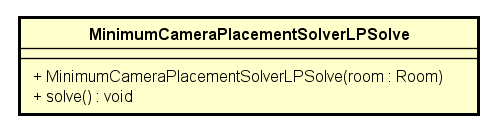
\includegraphics[scale=0.6]{class_minimum_camera_placement_solver_lp_solve}
	\caption[Diagram kelas \textit{MinimumCameraPlacementSolverLPSolve}]{Diagram kelas \textit{MinimumCameraPlacementSolverLPSolve}}
	\label{fig:class_minimum_camera_placement_solver_lp_solve}
\end{figure}

Kelas ini merepresentasikan pemecah masalah penempatan kamera CCTV dalam ruangan agar berjumlah minimum dengan menggunakan kakas \textit{lp{\_}solve}. Kelas ini merupakan turunan dari kelas MinimumCameraPlacementSolver. Diagram kelas \textit{MinimumCameraPlacementSolverLPSolve} dapat dilihat pada gambar~\ref{fig:class_minimum_camera_placement_solver_lp_solve}. Berikut ini merupakan fungsi-fungsi yang terdapat pada kelas \textit{MinimumCameraPlacementSolverLPSolve}:
\begin{itemize}
	\item \textbf{\textit{solve}() \(\rightarrow\) \textit{void}}\\
	Fungsi ini berguna untuk menyelesaikan masalah penempatan kamera CCTV dalam ruangan agar berjumlah minimum dengan menggunakan kakas \textit{lp{\_}solve}.
\end{itemize}











